\documentclass[12pt,letterpaper]{article}
\usepackage{graphicx,textcomp}
\usepackage{natbib}
\usepackage{setspace}
\usepackage{fullpage}
\usepackage{color}
\usepackage[reqno]{amsmath}
\usepackage{amsthm}
\usepackage{fancyvrb}
\usepackage{amssymb,enumerate}
\usepackage[all]{xy}
\usepackage{endnotes}
\usepackage{lscape}
\newtheorem{com}{Comment}
\usepackage{float}
\usepackage{hyperref}
\newtheorem{lem} {Lemma}
\newtheorem{prop}{Proposition}
\newtheorem{thm}{Theorem}
\newtheorem{defn}{Definition}
\newtheorem{cor}{Corollary}
\newtheorem{obs}{Observation}
\usepackage[compact]{titlesec}
\usepackage{dcolumn}
\usepackage{tikz}
\usetikzlibrary{arrows}
\usepackage{multirow}
\usepackage{xcolor}
\newcolumntype{.}{D{.}{.}{-1}}
\newcolumntype{d}[1]{D{.}{.}{#1}}
\definecolor{light-gray}{gray}{0.65}
\usepackage{url}
\usepackage{listings}
\usepackage{color}

\definecolor{codegreen}{rgb}{0,0.6,0}
\definecolor{codegray}{rgb}{0.5,0.5,0.5}
\definecolor{codepurple}{rgb}{0.58,0,0.82}
\definecolor{backcolour}{rgb}{0.95,0.95,0.92}

\lstdefinestyle{mystyle}{
	backgroundcolor=\color{backcolour},   
	commentstyle=\color{codegreen},
	keywordstyle=\color{magenta},
	numberstyle=\tiny\color{codegray},
	stringstyle=\color{codepurple},
	basicstyle=\footnotesize,
	breakatwhitespace=false,         
	breaklines=true,                 
	captionpos=b,                    
	keepspaces=true,                 
	numbers=left,                    
	numbersep=5pt,                  
	showspaces=false,                
	showstringspaces=false,
	showtabs=false,                  
	tabsize=2
}
\lstset{style=mystyle}
\newcommand{\Sref}[1]{Section~\ref{#1}}
\newtheorem{hyp}{Hypothesis}

\title{Problem Set 1}
\date{Due: October 1, 2021}
\author{Applied Stats/Quant Methods 1}

\begin{document}
	\maketitle
	
	\section*{Instructions}
	\begin{itemize}
		\item Please show your work! You may lose points by simply writing in the answer. If the problem requires you to execute commands in \texttt{R}, please include the code you used to get your answers. Please also include the \texttt{.R} file that contains your code. If you are not sure if work needs to be shown for a particular problem, please ask.
		\item Your homework should be submitted electronically on GitHub in \texttt{.pdf} form.
		\item This problem set is due before 8:00 on Friday October 1, 2021. No late assignments will be accepted.
		\item Total available points for this homework is 100.
	\end{itemize}
	
	\vspace{1cm}
	\section*{Question 1 (50 points): Education}

A school counselor was curious about the average of IQ of the students in her school and took a random sample of 25 students' IQ scores. The following is the data set:\\
\vspace{.5cm}

\lstinputlisting[language=R, firstline=40, lastline=40]{PS01.R}  

\vspace{1cm}

\begin{enumerate}
	\item Find a 90\% confidence interval for the average student IQ in the school.\\
	
	\item Next, the school counselor was curious  whether  the average student IQ in her school is higher than the average IQ score (100) among all the schools in the country.\\ 
	
	\noindent Using the same sample, conduct the appropriate hypothesis test with $\alpha=0.05$.
	\end{enumerate}
	
\section*{Problem 1 - My Answer (R code)}
	


\begin{lstlisting}[language=R]
#####################
# Problem 1 = My Answer
#####################

# Because the sample or n < 30 a t-distribution can be used as opposed to a normal distribution
#  t-distribution is a type of probability distribution. used where the sample size is small.

# The sample size is 25
y <- c(105, 69, 86, 100, 82, 111, 104, 110, 87, 108, 87, 90, 94, 113, 112, 98, 80, 97, 95, 111, 114, 89, 95, 126, 98)

# get the sample mean ( x bar) of y which is 98.44
n <- length(y) 
# sample mean
mean(y)
# standard deviation
sd(y)
(sd(y)/sqrt(n))
# CI of 90%
# From tables look for Degree of Freedom or DF of 24 and alpha level of 0.05
# this gives 1.71 or a t-score of 1.71
# 1. 25 - 1 = 24
# 2. 1 - .90 = .05 or the alpha level
# use alpha level of 0.05
c90 <- qt(.05, 24, lower.tail = FALSE)
c90
# CI tells us to take the mean of 98.44 and plus or minus 4.4778
lower <- mean(y) - c90*(sd(y)/sqrt(n))
upper <- mean(y) + c90*(sd(y)/sqrt(n))
# get the s or standard deviation of y which is 13.09287
#sd(y)
# Using a 90% confidence level and need to find the confidence interval
# Confidence Level or CI is the margin of error and written as ±
# CI is to do with how reliable the estimation is
# 1.71 * 13.09287 / square root of 25 = 4.4778
# 98.44 - 4.778 = 93.96 is the lower level
# 98.44 + 4.778 = 102.92 is the upper level
c(lower, upper)


# t test can be used for small samples
t.test(y)

\end{lstlisting}
	
\newpage

\section*{Problem 1 - My Answer  - R console output}
	

\begin{lstlisting}[language=R]

> # The sample size is 25
> y <- c(105, 69, 86, 100, 82, 111, 104, 110, 87, 108, 87, 90, 94, 113, 112, 98, 80, 97, 95, 111, 114, 89, 95, 126, 98)
> 
> # get the sample mean ( x bar) of y which is 98.44
> n <- length(y) 
> # sample mean
> mean(y)
[1] 98.44
> # standard deviation
> sd(y)
[1] 13.09287
> (sd(y)/sqrt(n))
[1] 2.618575
> # CI of 90%
> # From tables look for Degree of Freedom or DF of 24 and alpha level of 0.05
> # this gives 1.71 or a t-score of 1.71
> # 1. 25 - 1 = 24
> # 2. 1 - .90 = .05 or the alpha level
> # use alpha level of 0.05
> c90 <- qt(.05, 24, lower.tail = FALSE)
> c90
[1] 1.710882
> # CI tells us to take the mean of 98.44 and plus or minus 4.4778
> lower_lvl <- mean(y) - c90*(sd(y)/sqrt(n))
> upper_lvl <- mean(y) + c90*(sd(y)/sqrt(n))
> # get the s or standard deviation of y which is 13.09287
> #sd(y)
> # Using a 90% confidence level and need to find the confidence interval
> # Confidence Level or CI is the margin of error and written as ±
> # CI is to do with how reliable the estimation is
> # 1.71 * 13.09287 / square root of 25 = 4.4778
> # 98.44 - 4.778 = 93.96 is the lower level
> # 98.44 + 4.778 = 102.92 is the upper level
> c(lower_lvl, upper_lvl)
[1]  93.95993 102.92007
> # t test can be used for small samples
> t.test(y)
	One Sample t-test
data:  y
t = 37.593, df = 24, p-value < 2.2e-16
alternative hypothesis: true mean is not equal to 0
95 percent confidence interval:
  93.03553 103.84447
sample estimates:
mean of x 
    98.44 

\end{lstlisting}

\newpage

	\section*{Question 2 (50 points): Political Economy}

\noindent Researchers are curious about what affects the amount of money communities spend on addressing homelessness. The following variables constitute our data set about social welfare expenditures in the USA. \\
\vspace{.5cm}


\begin{tabular}{r|l}
	\texttt{State} &\emph{50 states in US} \\
	\texttt{Y} & \emph{per capita expenditure on shelters/housing assistance in state}\\
	\texttt{X1} &\emph{per capita personal income in state} \\
	\texttt{X2} &  \emph{Number of residents per 100,000 that are "financially insecure" in state}\\
	\texttt{X3} &  \emph{Number of people per thousand residing in urban areas in state} \\
	\texttt{Region} &  \emph{1=Northeast, 2= North Central, 3= South, 4=West} \\
\end{tabular}

\vspace{.5cm}
\noindent Explore the \texttt{expenditure} data set and import data into \texttt{R}.
\vspace{.5cm}
\lstinputlisting[language=R, firstline=54, lastline=54]{PS01.R}  
\vspace{.5cm}
\begin{itemize}

\item
Please plot the relationships among \emph{Y}, \emph{X1}, \emph{X2}, and \emph{X3}? What are the correlations among them (you just need to describe the graph and the relationships among them)?
\vspace{.5cm}
\item
Please plot the relationship between \emph{Y} and \emph{Region}? On average, which region has the highest per capita expenditure on housing assistance?
\vspace{.5cm}
\item
Please plot the relationship between \emph{Y} and \emph{X1}? Describe this graph and the relationship. Reproduce the above graph including one more variable \emph{Region} and display different regions with different types of symbols and colors.
\end{itemize}

\newpage

\section*{Problem 2 - My Answer (R code)}
	


\begin{lstlisting}[language=R]

#####################
# Problem 2 = My Answer
#####################

expenditure <- read.table("https://raw.githubusercontent.com/ASDS-TCD/StatsI_Fall2021/main/datasets/expenditure.txt", header=T)
str(expenditure)
# rows and columns 2 to 5
expenditure[2:5]

# This plots the relationships among Y, X1, X2, and X3
# using pairs() a matrix of scatter plots is produced
pairs(expenditure[2:5], main = "Correlation Matrix shown as a scatter plot")
# This shows that it is not correlated and is random

# Housing assistance and per capita expenditure / income
scatter.smooth(expenditure$Y, expenditure$X1, ylab="per capita income", xlab = "housing assistance")
# cor function calculates correlation among the vectors
# Region X1
# has the highest per capita on housing assistance
cor(expenditure$Y, expenditure$X1)
scatter.smooth(expenditure$Y, expenditure$X2)
# regions X2
cor(expenditure$Y, expenditure$X2)
scatter.smooth(expenditure$Y, expenditure$X3)
# Region X3
cor(expenditure$Y, expenditure$X3)
scatter.smooth(expenditure$X1, expenditure$X2)


\end{lstlisting}

 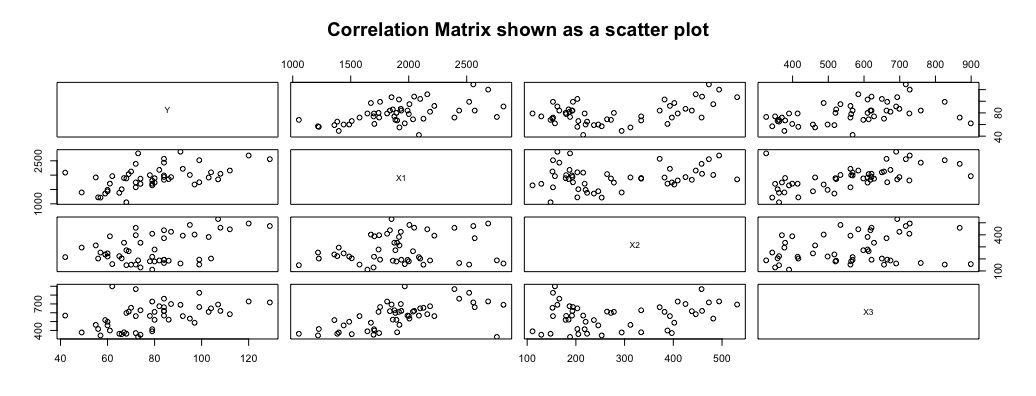
\includegraphics[width=\linewidth]{Rplot-marklkm.png}
 
  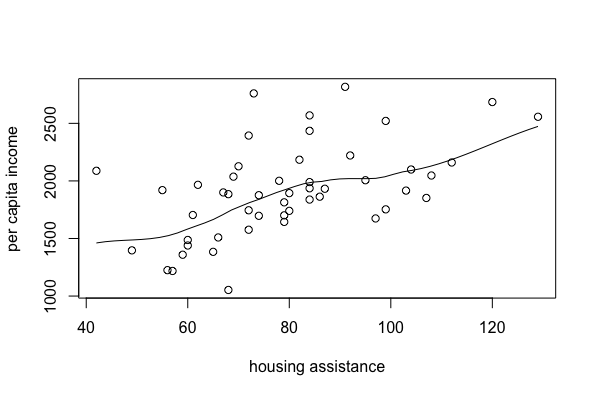
\includegraphics[width=\linewidth]{Scatter Smooth Rplot.png}


\end{figure}

\newpage

\section*{Problem 2 - My Answer  - R console output}
	

\begin{lstlisting}[language=R]

> expenditure <- read.table("https://raw.githubusercontent.com/ASDS-TCD/StatsI_Fall2021/main/datasets/expenditure.txt", header=T)
> str(expenditure)
'data.frame':	50 obs. of  6 variables:
 $ STATE : chr  "ME" "NH" "VT" "MA" ...
 $ Y     : int  61 68 72 72 62 91 120 99 70 82 ...
 $ X1    : int  1704 1885 1745 2394 1966 2817 2685 2521 2127 2184 ...
 $ X2    : int  388 272 397 458 157 162 494 153 152 187 ...
 $ X3    : int  399 598 370 868 899 690 728 826 656 674 ...
 $ Region: int  1 1 1 1 1 1 1 1 1 2 ...
> # rows and columns 2 to 5
> expenditure[2:5]
     Y   X1  X2  X3
1   61 1704 388 399
2   68 1885 272 598
3   72 1745 397 370
4   72 2394 458 868
5   62 1966 157 899
6   91 2817 162 690
7  120 2685 494 728
8   99 2521 153 826
9   70 2127 152 656
10  82 2184 187 674
11  84 1990 192 568
12  84 2435 166 759
13 104 2099 203 650
14  84 1936 193 621
15 103 1916 382 610
16  86 1863 185 522
17  69 2037 264 613
18  74 1697 129 351
19  79 1644 111 390
20  80 1894 179 520
21  78 2001 180 564
22  73 2760 188 326
23  92 2221 393 562
24  97 1674 402 487
25  66 1509 205 358
26  65 1384 223 362
27  57 1218 253 343
28  60 1487 220 498
29  74 1876 334 628
30  49 1397 294 377
31  60 1439 246 457
32  59 1359 237 517
33  68 1053 148 362
34  56 1225 203 416
35  72 1576 153 562
36  80 1740 278 610
37  79 1814 409 727
38  55 1920 312 463
39  79 1701 218 414
40  42 2088 215 568
41 108 2047 459 621
42  84 1838 438 618
43  87 1932 425 699
44  99 1753 194 665
45  84 2569 372 663
46 112 2160 446 584
47  95 2006 482 534
48 129 2557 473 717
49  67 1900 334 379
50 107 1852 531 693
> 
> # This plots the relationships among Y, X1, X2, and X3
> # using pairs() a matrix of scatter plots is produced
> pairs(expenditure[2:5], main = "Correlation Matrix shown as a scatter plot")
> # This shows that it is not correlated and is random
> 
> # Housing assistance and per capita expenditure / income
> scatter.smooth(expenditure$Y, expenditure$X1, ylab="per capita income", xlab = "housing assistance")
> # cor function calculates correlation among the vectors
> # Region X1
> # has the highest per capita on housing assistance
> cor(expenditure$Y, expenditure$X1)
[1] 0.5317212
> scatter.smooth(expenditure$Y, expenditure$X2)
> # regions X2
> cor(expenditure$Y, expenditure$X2)
[1] 0.4482876
> scatter.smooth(expenditure$Y, expenditure$X3)
> # Region X3
> cor(expenditure$Y, expenditure$X3)
[1] 0.4636787
> scatter.smooth(expenditure$X1, expenditure$X2)

\end{lstlisting}


\end{document}
